
\documentclass{report}

\usepackage{breakcites}

\usepackage{pdfpages}

\usepackage[margin=1.5in]{geometry}

\usepackage[utf8]{inputenc}
\usepackage [english]{babel}
\usepackage[autostyle, english = american]{csquotes}
\MakeOuterQuote{"}

\usepackage{listings}
\lstset{basicstyle=\ttfamily}

\usepackage{forest}

\usepackage{hyperref}

\author{Luke Jackson}
\title{Creating a Concurrent Compiler in Haskell}

\begin{document}


\maketitle

\begin{abstract}
Creating a compiler and virtual machine in Haskell to run Goal, a simple concurrent programming language of my own design based on Google Go. This dissertation can be treated as a introduction to implementing a compiler in Haskell, but a basic understanding of Haskell and Monads is assumed.
\end{abstract}

\tableofcontents


\chapter{Introduction \& Overview}

\section{Introduction To Project}

For my final year project I have created a compiler in Haskell for a simple programming language of my own design, which I based on Google's relatively new language Go. I called this language Goal, and it is a simplified version of Go but contains all of the features I was interested in implementing in my compiler, most importantly allowing concurrent programming.

The main focus of this project was to implement a parser, compiler and virtual machine for a modern concurrent programming language, not on designing a completely new language. Though I will briefly discuss the reasons behind creating Goal, it is important to understand the focus of this project is on compiler implementation using Haskell. Not on programming language design.

This document is split into five main sections; Designing Goal, Parsing, Code Generation \& Intermediate Representations, Code Execution and Testing. In each of these sections I will go into more detail about how I approached each of these problems. 

These next few pages will give a brief introduction to compilers and programming languages, also giving more information about Go and the motivation behind the project. I will also briefly discuss any development methodologies used and give a justification for certain technical decisions.

\subsection{Introduction to Compilers}

To understand what a compiler is, you need to first understand what a program is and, more importantly, what a programming language is. Programs have become a fundamental part of human existence. From performing simple calculations to creating applications that allow me to create documents such as this, they exist in every aspect of our life. For the simplest definition of what a program is, think of a program as a recipe.  

You have a list of resources that you need, followed by a series of instructions telling you what to do with these resources. Then, to run your program, you grab all the resources you need and follow the instructions.

Programs that run on computers have to be represented in someway that both humans and eventually computers can understand.  Therefore programs are written in programming languages, a good definition for programming languages can be found in  \cite[p,~1]{Comp2007}  where they state;

\begin{displayquote}
Programming Languages are notations for describing computations to people and machines … But, before a program (in this format) can be run it first must be translated into a form which can be executed by a computer.
\end{displayquote}

So this brings us nicely to being able to define what a compiler is. A compiler is something that takes programs written in one programming language and translates it into another programming language. Often taking a program written in a high level language, that humans write code in, and translating them into lower level languages that computers can more easily understand and then run.

This highlights the need for compilers, so that they can be used to translate high level languages into more easily executable lower level languages, that are much harder for humans to create programs in.

Finally a virtual machine is  a program that emulates a computer. In our case it is emulating a machine that is able to run code that has been compiled down to a low level instruction set. You will usually only see machines try to execute low level languages given the smaller, and more precisely defined, instruction set. As is the case with the virtual machine I have created. The benefit of creating a virtual machine to run your code is it allows you to run your code on any machine which can run your virtual machine. 

Looking at these explanations it is clear to see the importance of compilers and virtual machines in the modern world. They allow people to create complicated programs and applications efficiently without having to concern themselves with low level details.

\subsection{Introduction to My Project Structure}

There are three main parts to my compiler; parsing, compiling and the virtual machine. To best understand the structure of my compiler it is good to look at the definition of the function $run$ which is called to run Goal code.

\begin{lstlisting}
 	run f  = exec (typeChecker (comp (parseGo f)))
\end{lstlisting}

Where $f$ is the location of the .gol file we want to run. You can see that we first call the parser which passes its result to the code generator ($comp$), which passes its result to a simple type checker before the function $exec$ will run the compiled code. 

This shows how my compiler is structured and this dissertation will walk through the creation of the parser, code generator and virtual machine and how they interact with each other.

To run a program on my compiler you simply need to open and run the Haskell script GoalCompiler.lhs, then simply type the command $run$ followed by a sting containing the location of your .gol file. Then your code will be compiled and run. 

\subsection{Introduction to Goal}

Goal is the language I have created my compiler for. It is a language I have created specifically for this project as a means of exploring compilers. It draws heavy inspiration from Go and uses the same basic syntax where possible. The main features of Goal are the ability to perform function recursion and to create and run concurrent programs.

\begin{figure}[h]
\begin{lstlisting}
	global j = 20;
	
	func main() { 
	    var c chan = Make(chan int);
	    go pong();
	    go ping(j);
	    WaitOn(ping);
	    Kill();
	};
	
	func ping(n int) {
	    for (i = 0; i < n; i++) {
	        c <- 1;
	        Print("ping");
	    };    
	};
	
	func pong() {
	    for (True) {
	        WaitChan(c);
	        l = <- c;
	        Print("pong");
	    };    
	};
\end{lstlisting}
\caption{An example program in Goal, }
\label{fig:goalExample} 
\end{figure}

The idea for Goal came when I was picking features from Go I was interested in compiling then decided it would be a nice idea to bring them together to create a more complete language. In my opinion during the course of this project Goal has evolved from a means to explore compilers and language design into a simple standalone language with it's own uses. I will discuss more about the design and functionality of Goal in Chapter 2.

It is recommended to make use of the Goal Documentation found in the appendix when starting to write new programs in Goal. The provided documentation gives example syntax of every command you can use and provides examples of how to use them and explanations on how they are expected to behave.

\subsection{Introduction to Go}

Go is an object oriented programming language created by Google relatively recently in 2007. It is used by Google for many different applications, most notably it powers dl.google.com, a service which contains the source for Chrome and The Android SDK. A good place to find out more about the history of Go and it's development is in the documentation section on golang.org.

In many ways Go is similar to C in terms of syntax and that it is also statically typed. There are however some interesting features thrown in, such as how Go handles concurrency.

In summary I would say Go (also referred to as golang) is a new language with quite a bit of potential, which can be seen by it's growing popularity. Although it is not revolutionary, it's mixture of simplistic syntax and more exciting features makes it a good language to emulate.


\subsection{Introduction to Concurrency}

Concurrency is the primary feature I was interested in implementing in my compiler. It is a key part of this project and also a fundamental part of modern programming. 

The basic idea behind concurrent programming is you can do many things at one time. If we first define a sequential program as a sequence of operations carried out one at a time. We can then define a concurrent program as a program that contains a set of sequential processes executing in parallel \cite[p.~414]{CompGen1997}.

The importance of concurrent programming can be seen now more than ever with rising popularity of online services and cloud computing. Lets take one of the most popular websites in the world Google.com, with around 40,000 request a second there is a high chance that when you hit that search button, so are thousands of other people at exactly the same time. But instead of queuing every request and doing it sequentially a server will handle the requests concurrently, ensuring that many requests can be handled at the same time, and you don't have to wait for the thousands of people who clicked a few milliseconds ahead of you till you get your results.

There are plenty more examples of the importance of concurrency in modern technology, I'm sure if you think about most pieces of technology you use it would be easy to list numerous process that have to run concurrently. This is why I was interested in implementing concurrency into my compiler, because of it's usefulness and importance in modern programming languages.   

\section{Motivation}

The biggest motivation behind this project was a desire to learn more about compiling and executing modern object oriented programming languages. I was also curious about programming language design and wanted to take the chance to really look at a programming language analytically.

\subsection{Why Haskell}

I chose to implement my compiler using Haskell. Haskell is a purely functional language with strong static typing. Functional languages are often seen as good platforms to use when creating a compiler because some of their features make it easier to handle tree data structures, which can be important during parsing and creating an intermediate representation of language. Also the use of pattern matching and efficiently being able to recurse makes Haskell a good choice for implementing a compiler and a virtual machine.

Another reason I chose Haskell was quite simply that it is a language I enjoy working with, and more importantly for a project like this, would like to learn more about. I was keen with this project to not only create something interesting but also learn more about functional programming. I hoped to use this project to explore some  unique functional approaches to some of the problems creating a compiler can throw up. A good example of this is how I handled parsing and my use of Monadic Parser Combinators.

\subsection{Why Create A New Language}

There are so many great programming languages out there with fantastic supporting documentation that would be excellent choices to make compilers for. Which really begs the question, why did I go through the hassle of designing my own language to compile? The answer to this is pretty simple, with a project like this if I was to create a compiler for C++, for example, I would never have the time to create something that covers all of C++'s functionality within 9 months. Therefore no matter how well I had done with the project it would always feel a little incomplete, but more importantly if someone was to use my compiler they could very well end up trying to use features my compiler didn't support which would be frustrating for me and anyone who wishes to use my compiler in the future.

Instead of having this problem I decided I would create a new language that I could provide supporting documentation for and strictly define what is and isn't possible with in it. Because the focus of this project was not on language design my approach to creating a new programming language was finding a language I liked, then picking key features I was interested in exploring. Before finally adding some extra functionality so that this new language could be useful on its own.

The language I liked the look of was Go and that is where most of the features for my language came from, with the key feature I was interested in exploring being concurrency. I decided to call the language I had created Goal.

\subsection{Why Base This Language on Go} 

Go is not a language I was overly familiar with before the start of this project, but as soon as I looked into it I very much liked what I saw. 

At the start of this project I was exploring different possibilities of languages I could use as inspiration for Goal. When I came across Go I discovered it had a very clean and easy to understand way of creating and running concurrent process, which was one of the key features I was interested in putting into Goal. From there I began looking into Go's design and discovered not only did it have a wealth of interesting features to look at but also a clean and understandable syntax, which would work nicely with the simplistic easy to use nature I wanted to create in Goal.

The most important factors where defiantly the way Go handle concurrency and channels but also there was an aspect of using this project as a way of familiarizing myself with another language. It also helped that Go came with such a wealth of easy to navigate online resources which was perfect for when I needed to check the exact functionality of certain expressions.

Overall I felt Go provided me with a simple syntax and good implementations of the main features I was interested in implementing. Which made it a good choice to use as the basis of Goal.

\section{Development Process }

The main method I used for development was Test Driven Development (TDD). This is a simple approach where you write your test cases first, then write your code so that is passes all your tests. I found this to be quite an appropriate approach due to the iterative nature of my development process. 

I initially started work by focusing on being able to compile and execute a small subset of simple features such as if statements, variable assignments and simple arithmetic. Then using TDD I wrote tests for each new piece of functionality I wanted to add, expanding the subset of features I was able to handle. Due to the nature of TDD I was able to do this without worrying about breaking earlier features as I could just ensure all my original tests still passed.

As was mentioned before, I split the implementations of my compiler into three main sections;

\begin{itemize}
	\item Parsing
	\item Code Generation \& Intermediate Representations 
	\item Creating a Stack Based Virtual Machine
\end{itemize}

While developing my compiler and virtual machine I often found I would implement each feature in two steps; First ensuring I could create a suitable intermediate representation and updating my virtual machine to ensure it could handle the new feature. Then, once this was complete, I would update my parser to handle this new command. 

Often when working on multiple features at a time, it would be more efficient to update the code generation and virtual machine first for all the new features. Then update the parser second, rather than adding each new piece of functionality one at a time. 

I will go into more detail about the creation and running of my tests in Chapter 5. 
   

\chapter{Designing Goal}

This chapter deals with how I approached designing a new language and how I went about choosing the features I wished for Goal to contain. I will discuss some reasoning behind why certain features differ from how they are handled in Go and also talk about how I tried to make the language as complete as possible.

I think it is also important to note here that the main focus of this project is not on the design and creation of a new language but rather the implementation of the compiler itself.

\section{Picking Features}

As I mentioned before, rather than designing Goal from scratch I chose to instead choose features from Go I was interested in, then find a way of putting them into Goal. I did not create Goal with a target audience or with potential uses in mind, hence the lack of a specification or market research. Instead I created Goal as a means to let me implement a compiler that could handle a number of different interesting features.

Therefore you will find the features Goal can handle my seem quite varied and not completely complimentary of each other, but I do feel that Goal still has many uses. 

As much as Goal was created simply as a tool for creating an interesting compiler, I did also attempt to make it as user friendly as possible. I have created supporting documentation for Goal that has full examples of the syntax it uses and detailed explanations of how to use each of it's features.  
 
A good summary of my approach to creating Goal is that I filled it with features I wanted to explore, then added extra functionality to try and make the language as easy to use, complete and useful as possible.
 
\subsection{Syntax}

A language's syntax can be said to describe the form that commands and expressions in a language must take \cite[p.~72]{CompGen1997}. In the case of programming languages it defines how you must write your code so that it can perform the computations you wish.

The syntax for Goal is pretty simple and almost identical to that of Go, with some minor differences. I decided to follow Go's syntax rules not only for simplicity but also so it was easy to see where Goal got it's functionality from. I felt it would make sense to give it syntax rules close to the language it was emulating.
 
A key part of Goal's syntax is that each command must end with a semi-colon, including if statements, functions and for loops. A more detailed outline and examples of valid Goal syntax can be seen in the accompanying documentation for Goal with examples of syntactically correct Goal \cite{GoalDoc}. 

\subsection{Types}

\subsection{Basic Commands}

\subsection{Functions}

\subsection{Concurrency}



\section{Differences From Go}

\section{Possible Uses}


\chapter{Parsing}

Parsing is a fundamental part of compiling, you can think of it as the front end of the compiler. In simplistic terms it takes in a program as raw text and then builds a data structure that represents the program the user has written. In my project the raw text is the code from a .gol file and the data structure is the intermediate representation of Goal. 

Although I will be talking a lot about the intermediate representation I've created to parse my text into, I will not be going into much detail about the design of that data structure. That is covered in more detail in the next chapter. In this section a preexisting understanding of Monads in Haskell is assumed.      

\section[Introduction to Using Monadic Parser Combinators]{Introduction to Using \\ Monadic Parser Combinators}

The technique I used to parse data in my compiler was to make use of Monadic Parser Combinators. If we think of a parser in Haskell as something that takes in a string and returns a data structure, we can think of parser combinators as high order functions that take in several parsers as its input and returns a new parser as it's output.  

\section{Goal Syntax Rules and Justifications}

As was discussed in the previous structure Goal gets most of its syntax rules from Go. There are however some unique syntax rules I decided to implement in Goal that you will not find in Go. There were two main reasons why syntax rules my differ from Go. 

The first being it was a design choice. For example if you look at variable declaration in Go it can be done one of 2 ways.

\begin{lstlisting}
	var i int = 42
	j := 42
\end{lstlisting}    

Although I could have implemented variable declarations to look like this I decided because variables can be declared on the fly and because of the simplistic nature of my type system I may as well keep declarations and assignments the same, and as simple as possible. Hence in Goal all you need to write to declare or assign a variable is;

\begin{lstlisting}
	l = 42;
\end{lstlisting}
 
There are several examples of these changes in syntax for design choice, such as global variable definitions and the requirement of brackets to hold conditional statements. These small changes where made merely as a way to tidy up Goal and make it have a more complete and consistent syntax. 

The other reason Goal's syntax varies from Go is because of the limitations within the implementation of my parser. 

For example, in Go you don't need to use semi colons at the end of a command. Where as I decided that in Goal I would make it necessary to include semi colons at the end of every command, including if statements and function declarations. For example;

\begin{lstlisting}
	func main() {
	    i = 2;
	    j = 0;
	    for (i < 100){
	        i = square(i);
	        j ++;
	    };
	    Show(j);		
	};
	
	func square(n int) int {
		return n * n;
	};
\end{lstlisting}

You can see in this simple program how every command even function definitions and for loops need to finish with a semi colon.

This is because it makes it easier to split up commands based on every time I see a semi colon. The reasons I made some of these choices was not because it was not possible for me to implement different syntax rules, but because the main focus of this project was not on parsing and if a small change to syntax meant a quicker implementation sometimes I felt it necessary. 


\section{Parser Implementation}

My parser implementation was focused around using monadic parser combinators. As part of this I used a collection of functions provided from the paper. %TODO Cite Graham's paper % 
These can be seen in my abstract in the Parsing.lhs file. What these functions do is provide a series of simple parsers to use when creating more complicated parser combinators. 

Then it was simply a question of building up parsers to handle more restrictive rules. A good way to understand this is to walk through a simple example of parsing comparative expressions. 

Although this section gives a walk through of how I used parser combinators, it should not be considered a standalone introduction. The interested reader should look at %TODO cite paper % 
which provides a more in depth introduction and more detailed descriptions about monadic parser combinators.

\newpage

\subsection{Example of Parser Implementation}

If we first start with defining the data structure, also known as the intermediate representation we wish to parse down to, we can then look to define the language which we are parsing;

%TODO check all code works
\begin{lstlisting}
data Expr 	= CompExpr Op Expr Expr | Val Number
	
data Op		= EQU | NEQ 
	
type Number	= Int 
\end{lstlisting}

This is a pretty simple data structure representing two types of conditional expressions. We now need to define a grammar that is acceptable for our language. A grammar, or formal grammar, is a set of rules by which valid sentences (or in our case commands and expressions) in a language are constructed \footnotemark[1].  In this case when we talk about a language we are not talking about a programming language in the typical sense, instead we define a language as a set of strings made of symbols that our limited by rules that are specific to that language \footnotemark[2]. 

\footnotetext[1]{\url{http://dragonbook.stanford.edu/lecture-notes/Stanford-CS143/06-Formal-Grammars.pdf}}
\footnotetext[2]{\url{http://en.wikipedia.org/wiki/Formal_language}}

To define our grammar it is good to look at some examples of what is acceptable in our little language, if we say we are only interested at looking at conditionals where you use $==$ to signify equals and $!=$ to signify two values being not equal;

\begin{lstlisting}
	4 == 7
	5 != 5
	42 == 42
	12 != 34 
\end{lstlisting}

You may notice that the expressions we are allowing don't have to be true. In this example we are allowing the user to express comparative expressions our parser has no need to deal with what is and isn't allowed computationally as long as our grammar allows it, the expression can be as bizarre as you want. This shows how we have to be careful defining our grammar to only allow what we want. For example if we look at our data structures we actually allow for some nested comparisons.

\newpage

You can see that in our data structure the following expression is valid;

\begin{lstlisting}
CompOp EQU 
	(CompOp NEQ 
		(Val 5) 
		(CompOP EQU 
			(Val 4)
			(Val 7))) 
	(CompOp NEQ 
		(Val 3) 
		(Val 5))
\end{lstlisting}

Which would look like this;

\begin{lstlisting}
 (5 != (4 == 7)) == (3 == 5)
\end{lstlisting}

Now you can argue this makes sense and should be allowed but I feel like in our simple language it's not what we want to include, also we need to consider if we end up including more types of comparisons, such as $>$ or $\geq$. Things will start to get messy quickly. Regardless of the justification for this example we won't allow nested comparisons. 

There are two ways to handle this problem. We can either alter our data structure so that it is no longer allowed, or we can create a grammar that does not allow for nested comparisons in our language. It is better to restrict our grammar than our intermediate representation. So we now need to define our grammar. In simple terms we can describe it as;

\begin{lstlisting}
 <NUMBER1> <COPARISON OPERATION> <NUMBER1>
\end{lstlisting}   	

Though we need to create a more formal definition. Lets say a sentence in our language has to consist of one natural number followed by either a $==$ or $!=$ then another natural number. We will allow white space between the numbers and comparison operators.By natural numbers we are referring to any whole number. 

To create a parser to handle this grammar we will need to make use of some parsers provided in Parsing.lhs;

\begin{itemize}
\item $natural$, will parse natural numbers
\item $symbol s$ will parse the given symbol s 
\end{itemize}

Making use of this we can use of Haskell's do notation we can also generate a parser to parse the different conditional symbols $==$ and $!=$. 

\begin{lstlisting}
	parseOp   :: Parser Op
	parseOp   = do symbol "=="
	               return (EQU)
        	     +++ do symbol "!="
	                    return (NEQ) 
\end{lstlisting} 

Using parse combinators means we can combine multiple parsers. Using this approach we can now create code to evaluate conditional expressions allowed in our language;

%TODO check all this code
\begin{lstlisting}

evalCompExpr    :: String -> Expr
evalCompExpr xs = case (parse compExpr xs) of
                    [(e,[])]  -> e
                    [(_,o)]   -> error ("unused "++ o)
                    []        -> error "invalid"

parseComp        :: Parser Expr	
parseComp        = do n1 <- natural
                      o  <- parseOp 
                      n2 <- natural
                      return (CompOp o n1 n2)  
\end{lstlisting}

This example shows how you build a simple parser using monadic parser combinators and the Haskell script provided %TODO cite grahams paper %
. It shows the the process of building up a grammar to define your language and also begins to show the process of combing parsers. 


\subsection{Analysis and Expansion of Parser Example}

Looking at this example you can see the process of slowly building up a grammar and the parsers to enforce it.

There are a number of important ideas shown in this example, one of the most important concepts is the idea of making sure your parser is more restrictive than your data structure. There are several aspects of my intermediate representation that allow for features that are restricted in my grammar. The reason this is done is because it makes generating code simpler without really making my parser any more complex.  

Another good thing too take away from this is the idea of abstracting problems out our final parser could have easily looked like this;

\begin{lstlisting}
parseComp        :: Parser Expr	
parseComp        = do n1 <- natural
                      do symbol "==" 
                         n2 <- natural
                         return (CompOp EQU n1 n2)
                       +++ do symbol "!="
                              n3 <- natural
                              return (CompOp NEQ n1 n3)
\end{lstlisting}

But because of the creation of our $parseOp$ function not only were we able to have a much cleaner implementation, also making it  much easier to expand our parser to include more comparison operations.

One concept that is not touched upon in this example is the idea of having a hierarchy of bindings. If we take the idea of operator precedences within mathematical expressions if we want a multiplication to be done before an addition in our language we need to generate an intermediate representation that will show this.

By combining multiple parsers we can create a hierarchy were an addition expression is dealt with before anything else by splitting on the $+$ symbol before anything else. Then nesting other arithmetic expressions within the output of the first parser. Examples of this technique can be seen throughout the implementation of my parser.


\section{Potential for Expansion}

Parsing is a topic that could easily become the main focus of a project like this. The idea behind using parser combinators was that they had been something I was interested in exploring and the more i used them the more I began to see how they could take up ore of this project. Instead I decided to focus this project in other areas but that does leave a list of areas I would be interested in coming back too. 

One of the main things you could expand within my parser would be to add some lexical analysis before beginning parsing. Lexical analysis is used to identify a valid set of words used in the language \cite[p.~13]{CompDes2005}. It is useful a it means you don not begin actually parsing before being certain that only valid commands exist in each program.

Another big area for expansion would have been spending more time looking into being able to add more types. You will notice looking at my code that my compiler and executor can handle doubles. But unfortunately due to limitations with my parsing I was decided against including it in the final release of Goal because I wanted to focus more time elsewhere. Though if this project was picked up in the future it would be one of the first features to update.    

   
 

\chapter{Code Generation \& Intermediate Representation}

Code generation is where I take the parsed input and then generate code from a low level instruction set that can then be executed. I decided to implement my own low level language and create an executor alongside that. Thus meaning that I would be compiling the parsed input down to code that used an instruction set that I had defined.

A key part of this section is looking at how I designed and implemented an intermediate representation of Goal in the form of a data structure. This intermediate representation was then simpler to compile into my low level instruction set. The importance of a good intermediate representation can be seen in \cite[p.~221]{EngComp2012} where they state;

\begin{displayquote}
Most passes in the compiler read and manipulate the IR form of code. Thus, decisions about what to represent and how to represent it play a  crucial role in both the cost of compilation and it's effectiveness. 
\end{displayquote}

In this section I will go into detail about the design of the data structure that you are required to parse down to, and which represents all of the features I implemented in my language. I will also be discussing some of the more interesting features that I implemented and how they were dealt with by the code generator.

Although in this section I will be talking a lot about code generated using the instruction set defined in my executer, I will not be going into detail about the design of the executor or the low level language I created. For more information on this you can go to the next section that does focus more on the design and execution of the low level instruction set.


\section{Intermediate Representation}

Having a good intermediate representation of the program being compiled is very important part of creating a compiler. It is important to make sure that you do not misinterpret the program you are compiling and a good way to do this is to create a data structure that clearly represents what your program is doing, whilst ensuring this data structure is easy enough to compile into your target language.

\subsection{Introduction to Intermediate Representations}

An intermediate representation of a program is where you create some data structure of your program that can be more easily interpreted and handled by your compiler. It is also important to ensure your IR\footnotemark[1] is designed in such a way that you capture the meaning of the program you wish to represent, and do not end up misrepresenting your program.

\footnotetext[1]{IR is shorthand for Intermediate Representation}

There are several approaches to generating an IR. These can been seen in \cite[p.~223]{EngComp2012} where they state there are three main approaches to generating an IR; 

\begin{itemize}
\item Graphical IRs, This uses tree or graph data structures.  
\item Linear IRS, This will closely resemble pseudo-code. 
\item Hybrid IRS, A combination of both Linear and Graphical approaches.
\end{itemize}

I chose to go with a Hybrid IR. A most suitable approach for me because, as stated in \cite[p.~113]{CompDes2005}, Linear IR are often used when compiling for stack base virtual machines, which is the architecture of the virtual machine that I created. But also this approached allowed me to take advantage of how easily Haskell allows you to create recursive data structures, that can be used when generating trees you would find in Graphical IRs.  

This approach provided me with a relatively high level representation of programs, meaning it gave a representation that would closely resemble the pseudo-code of the program you are trying to compile. This makes it nice format to work with as it makes it easier to visualize what is actually occurring during the later stages of code generation. 

It is important to note there are several different approaches I could have used when creating an intermediate representation and the choice to use a high level approach was both a design choice and also to do with ease of implementation. 

To best understand the approach I used to create the data structure for my intermediate representation it is good to follow a simple example of how you take a specific command then translate that into my intermediate representation.

\subsection{Example Creating an Intermediate Representation}

I will now show an example of the process I went through when generating my IR. The example I will use is creating a data structure that best represents an if statement. This is what an if statement looks like in Goal;

\begin{lstlisting}
	if (x < 1) {
		return x;
	};
\end{lstlisting}

You can see that there are two main parts to this statement. The condition directly after the if command,  $(x > 1)$  and then the code ,in this case $return$ $x;$, inside of the curly brackets. 

What is important to notice is that you could replace the return statement with any other acceptable code, even another If statement. Whereas the expression after the if is limited only to be certain things. In this case we could rewrite a general definition for an if statement to look like this;

\begin{lstlisting}
	if EXPRESSION {
		PROGRAM 
	}
\end{lstlisting}

This can be described by saying; If some expression is true, then execute the program inside the curly brackets.
 
Now all we need to do is define what  EXPRESSION and PROGRAM can be. Then we can create a data type in Haskell code to represent If statements that looks like this;

\begin{lstlisting}
	data IfStatement = If Expr Prog 
\end{lstlisting}

A program is quite easy to define, it's just a one or more instructions written to perform a specific task\footnotemark[2]. Therefore we must define all of the instructions that can be used to make a program in our data type Prog. Looking at our example that needs to include return statements, but I also said we were allowed to have nested if statements. Therefore we can create a recursive data structure that will allow this;

\footnotetext[2]{$wikipedia.org/wiki/Computer_program$}

\begin{lstlisting}
	data Prog = If Expr Prog | Return Expr
\end{lstlisting}


An expression is slightly harder to define. In the case of If statements we know our expression needs to do something. It needs to give us some condition which we can then decide is true or false. 

We can now create a data type for our expressions. We will need to allow for nested expressions but also allow for different comparison operators such as equals or less than. This can be shown here;

\newpage

\begin{lstlisting}
	data Expr = ExprComp Op Expr Expr 
                  	| Val Number 
                 	| Var Name
 
	data Op	  = GET | LET | NEQ | EQU
\end{lstlisting}

Although this example gives us quite a strict definition of what an expression needs to be for an If statement later on we will need to come up with a more general definition that is more applicable to other instances of using expressions (such as in arithmetic operations). The language specification for Go describes an expression by saying; "An expression specifies the computation of a value by applying operators and functions to operators". Another way to think of an expression is it is any valid unit of code that resolves to a single value \footnotemark[3].

\footnote[3]{url for quote}

Now that we have our definitions for what Expressions and Programs can be, we can begin to group what instructions belong in which section. With all our expressions being defined in the data type Expr and all our instructions used to make programs in the data type Prog.

Therefore if we are only considering our If statement example from earlier (ignoring how we defined the variable  x) we end up with the following data structure;

\begin{lstlisting}
	data Prog   = If Expr Prog | Return Expr

	data Expr   = ExprComp Op Expr Expr 
	               |Val Number 
	               |Var Name 

	data Op     = GET | LET | NEQ | EQU

	type Name   = Char

	type Number = Int
\end{lstlisting}

The above data structure now enables you to create high level intermediate representation of the original If statement we looked at, through the use of Haskell data types. 

You can see here how the data structure has a broad scope actually allowing expressions such as $(4<6) != (4 < (5>6))$, which don't really make sense. But I felt it was better to allow for these bizarre expressions, and handle any stricter rules in parsing stages. Rather than create an IR that was too restrictive.

\subsection{Analysis and Expansion of Creating an IR Example}

The key point of the above example is to understand that each part of a languages features can be, and needs to be, strictly defined. I found it important to remember the data structure I am creating  has a purpose other than just being a new representation of Goal. It needs to actually extract the important pieces of information from the code, such that you are left with a series of concise statements that hold all the information necessary for you to start to rebuild the program using a new instruction set.

The example also highlights the process of abstracting out each part of a languages functionality, then choosing the appropriate structure to use to represent them. An important part of this example is showing the use of recursive data structures to generate tree like data types.

For example look at the code;

\begin{lstlisting}
	if (x > 1){
		if (x > 5){
		 	if (x == 6) {
		 		return 1;
		 	};	
		};
	};
\end{lstlisting}  
 
It will be represented using data structure from our example by the following Haskell expression;

\begin{lstlisting}
If (ExprComp GET (Var 'x') (Val 1)) 
	(If (ExprComp GET (Var 'x') (Val 5))
		(If (ExprComp EQU (Var 'x') (Val 6))
			(Return (Val 1)))) 
\end{lstlisting} 

This can also be visualized in a tree structure with branches to the right being the outcome if the condition is true and branches to the left if the condition is false;

\begin{figure}[h]
\centering
\begin{forest}
for tree={
  draw,
  minimum width=3cm, 
  minimum height=1cm,
  anchor=north,
  align=center,
  child anchor=north
},
[{$x > 1$}, align=center
  [{$break;$}]
  [{$x > 5$}
    [{$break;$}]
    [{$x == 6$}
  		[$break$]
  		[$return$ $1;$] 
  	]
  ]
]
\end{forest}
\caption{Visual representation of tree structure of nested if statements}
\label{fig:ifTree} 
\end{figure}

What figure~\ref{fig:ifTree} shows you is the importance of using recursive data structures when allowing an arbitrary number of nested commands. You will see that as you start to expand your data structure to include multiple function declarations, or even large conditional expressions, building a tree like data structure is a good way to represent any program.

Overall this example helps to introduce all the key concepts behind the creation of the IR I used in my compiler.

\subsection{My Intermediate Representation of Goal}




\subsection{Handling More Complex Features in my IR }

\section{Code Generation}

\subsection{Introduction to Code Generation}

\subsection{Brief Introduction to Target Language Instruction Set}

\subsection{Example Code Generation}

\subsection{Analysis and Expansion of Code Generation Example}

\subsection{Examples of Generating Code For More Complex Features}

\chapter{Code Execution using a Stack Based Virtual Machine}

This chapter goes into detail about the method I used to execute the code generated by the code generator. The previous sections have mainly focused on compiling programs down to an instruction set. In this section I will go into detail about the design of that instruction set and the method I used to run it.

When creating a compiler you must take in a source language, the code you wish to compile, and then output a target language. A target language is the language you wish to compile into. In simpler terms, your compiler is taking in programs in your source language and then outputting the same programs but they are now represented using your target language.    

For a project like this there are two approaches you can take when choosing what your target language should be. You can either find a preexisting low level language like ARM code or Java Byte Code. Or you can create your own instruction set and a virtual machine that is capable of executing those instructions. I decided to make my own instruction set and a virtual machine to execute it. 


\section[Introduction to Stack Based Virtual Machines]{Introduction to \\ Stack Based Virtual Machines}

There are two things too define here before we can start talking about stacked based virtual machines . We need to first define what is a virtual machine, then secondly what is a stack machine. 

A virtual machine can be described as a self contained operating environment that behaves as if it is a separate computer\footnotemark[1] . This can be useful because it means no matter what machine you are running your VM\footnotemark[2] on any application you run on your VM will run the same regardless of the physical machine you are using.

\footnotetext[1]{\url{http://www.webopedia.com/TERM/V/virtual_machine.html}}
\footnotetext[2]{VM is short hand for virtual machine}

A good example of a virtual machine is if you have ever played a retro games console emulators on your phone or computers. Those are examples of fully functional virtual machines running old programs independently of the machine they are running on. 

A stack machine is a machine or (virtual machine) that uses a pushdown stack instead of set registers to evaluate different expressions\footnotemark[3]. A pushdown stack is a data structure with two main operations;
%TODO reference intro to algo here % 

\begin{itemize}
\item Push, which puts something onto the stack.
\item Pop, which removes the last element put on to the stack.
\end{itemize} 

%Maybe chnage this analagy%
You can think of a stack like a PEZ sweet dispenser. The first bit of candy you put in goes straight to the bottom of your dispenser and if you put more in they get pilled in on top. This is the same way you push objects onto a stack. Then when you wish to eat your candy, the last piece you put in comes back out first. This is the equivalent of popping the stack where the last object you pushed onto the stack comes out first. This is called a last in first out system.    

\footnotetext[3]{\url{http://en.wikipedia.org/wiki/Stack_machine}}

Therefore a stack machine is quite simply a machine that uses a stack instead of allocated registers to handle expressions. If you look at %figure~\ref{fig:stackExample}% 
it shows you how the expression $2 - 1$ would be evaluated using a stack in a stack machine.

Now we understand what a stack machine is and what a virtual machine is it becomes quite easy to understand what a stack based virtual machine is. Quite simply it is a virtual machine that uses a stack architecture, effectively you can think of the virtual machine I created as a simple stack machine emulator. 


\section[Implementing a Stack Based Virtual Machine]{Implementing a Stack Based \\ Virtual Machine in Haskell}

The way the executor I crated works is it takes in code written from a simple instruction set then the virtual machine will execute the code one instruction at a time. For a quick overview of how my stack based virtual machine works you can look at the type of the main functions that handle executing code.

\begin{lstlisting}
	exec	:: Code -> String
\end{lstlisting}

Which simply starts a call to the recursive function;

\begin{lstlisting}
	exec' 	::exec' type goes here 
\end{lstlisting}

\newpage

What looking at $exec$ shows is all that is needed to start the executor is the code that has been generated by the code generator. Then looking at $exec'$ you can see the different data structures that are used in implementing my virtual machine in my executor. The main components are;

\begin{itemize}
\item The Code
\item The Program Counter
\item The Stack
\item Memory
\item Channels
\item List of Subroutines
\end{itemize}

The code is simply referring to the code you are currently executing and the program counter tells you where in that code you are. The stack is used like registers would be, where you will hold values you are currently interested in handling. Memory is where you store any variables that you will need to refer back to. Subroutines and channels are used for concurrency and I will go into more detail about them later. 

The key concept to take way is that memory is for storing objects for the long term where as the stack is for passing around values and holding them temporarily.

\subsection{Explanation of Instruction Set}

\begin{figure}[h]
\centering
\begin{lstlisting}

	data Inst  = PUSH Number
	              | PUSHV Name
	              | POP Name
	              | SHOW
	              | PRINT String  
      		      | DO ArthOp
       		      | COMP CompOp
       		      | JUMP Label
      		      | JUMPZ Label
      		      | LABEL Label
      		      | FUNC FName
      		      | FEND
      		      | VCALL Name
      		      | CALL Name
      		      | STOP
      		      | RSTOP
      		      | MAIN
      		      | PUSHC Name
      		      | POPC Name
      		      | CHANNEL Name
      		      | WAIT
      		      | KILL
      		      | GO Name 
	
	type Label =  Int


\end{lstlisting}
\caption{Haskell data structure used to represent all the instructions in my instruction set.}
\label{fig:instData} 
\end{figure}

Chapter 4 shows how the code is generated from an instruction set, and in figure~\ref{fig:instData} you can see the data structure I created in Haskell that represents my instruction set. 

To understand how this instruction set works it is good too look at a couple of examples of generated code from the instruction set and what exactly different instructions mean. Then we can move on to looking at more detailed example of how you go about building an executor for this instruction set in Haskell. 

If we first look at a variable assignment. If we wanted to compile the code: $x = 7;$ it becomes;

\begin{lstlisting}
	PUSH (Integer 7)
	POP "x"
\end{lstlisting}

Or more accurately in Haskell, since Code has the type $[Inst]$, it would look like this;

\begin{lstlisting}
	[PUSH (Integer 7), POP "x"]
\end{lstlisting}

This uses two of the most important instructions. $PUSH$ Takes a number as an argument and pushes it onto the stack, $POP$ takes a name as an argument and removes the head of the stack saving it in memory, overwriting any existing variables with the same name in the same scope in memory. You can use $PUSHV$ which takes a name as argument to push a variable from memory onto the stack. 

In code generation one of the few features of the instruction set I went into in any detail was the idea behind the $LABEL$ and $JUMP$ instructions. So you may remember that compiled code for the expression;

\begin{lstlisting}
	for (x < 5) {
		x++;
	};
\end{lstlisting}

Will look like this;

\begin{lstlisting}
	[LABEL 0, PUSHV "x", PUSH (Integer 5), COMP LET, 
	JUMPZ 1, PUSHV "x", PUSH (Integer 1), DO ADD, 
	JUMP 0, LABEL 1]			
\end{lstlisting}

To understand this better we can annotate the code to show what is going on at each instruction, this is shown in figure~\ref{fig:whileExp}. It is a good way to explain several instructions that I will be using frequently throughout this chapter.

\begin{figure}[h]
\centering
\begin{lstlisting}[basicstyle=\ttfamily\small]
LABEL 0	         -- places a label with name 0 

PUSHV "x"        -- pushes variable x onto the stack 

PUSH (Integer 5) -- pushes the number 5 onto the stack 

                    performs "<" comparison between the 
COMP LET         -- top 2 elements of the stack, places 0 
                    ontop of the stack if it's false and 
                    1 if true   
	                    
JUMPZ 1          -- jumps to label 1 if the head of the 
                    stack is 0 
	
PUSHV "x"        -- pushes varaible x onto the stack
	
PUSH (Integer 1) -- pushes number 1 onto the stack
	
DO ADD           -- adds the top two items on top of the
                    stack, places result on top of stack

POP "x"          -- pops the item from top of stack and
                    saves it memory with name "x"

JUMP 0           -- Jumps to the label 0         

LABEL 1          -- places label 1 			
\end{lstlisting}
\caption{Annotated example of what each instruction is doing in a simple while loop}
\label{fig:whileExp} 
\end{figure}

This gives a more detailed insight into how $JUMP$, $JUMPZ$ and $LABEL$ are used to represent conditional expressions on a lower level. It also introduces the idea of how you perform operations involving two values, where you have instructions that pop the top two elements of the stack then push the result of the operation back onto the stack.

\subsection{Example Virtual Machine}
\label{sec:exmpCodeExec}
I will now run through an example of how I created a virtual machine to handle my instruction set. To do this I will start with a data structure representing a much smaller set of instructions and then show how I build a virtual machine capable of executing code built from these instructions.

The instructions I will use in my example can be shown in the following data structure;

\begin{lstlisting}
	data Inst  = PUSH Number
	              | PUSHV Name
	              | POP Name
      		      | DO ArthOp
       		      | JUMP Label
      		      | JUMPZ Label
      		      | LABEL Label
\end{lstlisting} 

This is a relatively small set of instructions in comparison to what I used in my final project, but you should be familiar with most of the commands, as they were all introduced in the previous section. 

Now we have our instruction set we can move on to defining everything we will need to make it work.

\begin{lstlisting}
	type Name   = String
	
	type Number = Int
	
	type Label  = Int
	
	data ArthOp = ADD | SUB 
\end{lstlisting} 

Now we have some raw data types to use, we now need to think about what we will need in our virtual machine to make it work. For this example we will definitely need a memory and a stack. So we add;

\begin{lstlisting}
	type Code    = [Inst]
	
	type Stack   = [Number]
	
	type Memory  = [(Name, Number)]		
\end{lstlisting} 

It make sense that memory should be a list of tuples because memory is a series of values with an allocated name used to reference them. It also makes sense that our Stack just needs to be a list of numbers. We now need to decide what our executors type should be. I think its good if it takes in some code and returns us the stack. But the problem with that is how do we pass about all the components of our virtual machine. well we need too create a helper function thats going to do all the hard work. Seeing as we just need the code to start our executor we can write;

\begin{lstlisting}
exec     :: Code Stack
exec c   = exec' c 0 [] []

exec'    :: Code -> Int -> Stack -> Memory -> Stack	
\end{lstlisting} 

So now we need to decide how we will handle our code. If our code is just a list of instructions then we can use our program counter to find the element in the list we should be dealing with then use a case analysis to say what to do depending on our instruction.

Lets pretends we have already defined some functions to speed things up. 
\begin{itemize}
\item $pop$ will take in the stack and return the stack after popping it
\item $push$ will take in the stack and a value, pushing that value to the top of the stack, then returning the updated stack
\item $pushv$ will do the same as $push$ but takes in a name and memory and pushes the variable from memory to the stack
\item $save$ will take the head of the stack and a name, then save that value to memory
\item $jump$ will take in the code and a label number and return a program counter that is set to the location of that label.
\item $jumpz$ does the same as $jump$ but takes in the stack as well only performing a jump if the head of the stack is 0, otherwise it just increments the program counter as normal.
\end{itemize}

 
We will also need to define a function $do$ that will take take in the stack and an $ArthOp$. Then it will return the stack after performing the required operation on the top two elements of the stack and pushing the result on top. I will define this function below as an example, so as to give you an idea as to how some of the other functions could be implemented.

\begin{lstlisting}
  do      :: ArthOp -> Stack -> Stack
  do o s  = case o of
               ADD -> push (v2 + v1) ns 
               SUB -> push (v2 - v1) ns
            where 
               v1   = head s
               v2   = head (tail s)
               ns   = (pop (pop s)) 
\end{lstlisting}

\newpage

Now that we have these functions we can easily create a recursive function to handle a long list of instructions. 

\begin{lstlisting}[basicstyle=\ttfamily\small]
exec'     :: Code -> Int -> Stack -> Memory -> Stack
exec'c pc s m 
          = if pc >= (length s) then s 
            else 
              case c !! pc of
                POP n    -> exec' c (pc+1) (pop s) (save s m)
                PUSH v   -> exec' c (pc+1) (push v s) m
                PUSHV n  -> exec' c (pc+1) (pushv n m s) m
                LABEL l  -> exec' c (pc+1) s m
                JUMP l   -> exec' c (jump l c) s m
                JUMPZ l  -> exec' c (jumpz l c s) (pop s) m
                DO o     -> exec' c (pc+1) (do o s) m               
\end{lstlisting}

The above function is a very basic example of how the main function in my executor works. Using recursion and pattern matching I am able to iterate over a list of instructions and create multiple functions to assist me in creating an efficient implementation of a virtual machine.  

\section{Handling More Advanced Features}

After using the example to show you how my executor works, I will now discuss some of the more interesting features I implemented in my executor and how I handled these features. 

\subsection{Memory Design and Implementation}

Memory is handled very simply in this project it has the same type it was given in the example in section \ref{sec:exmpCodeExec} and variables are referenced in almost exactly the same manner. The only major difference is that I included variable scope in my project and as such had to handle a number of different possible outcomes.

\subsubsection{Handling Variable Scope}

The main difference from the example is that memory in my executor is partitioned when it is initialized. My parser does not allow for variables the empty string as the name. Therefore to partition memory I initiate memory by creating a list of ten empty values , $("",0)$. Then all global memory is stored at the head of the list and local memory is stored at the tail, meaning memory is split in two. This makes it easy to handle scope because every time there is a change of scope, e.g. you begin to execute a function, you can simply drop everything after the list of empty variables as they will no longer be in scope.
  
This is a very simple approach to partitioning memory and one of the weaker aspects of this project. The current implementation does not facilitate the use of pointers, due to the complete dropping of the previous local memory  on a change of scope, but this would not be too difficult to update my executor to handle. Though it may require restructuring the way I currently handle memory.  


\subsection{Stack Management}

Manging a stack is a very important part of implementing an efficient and, more importantly, working stack based virtual machine. 

\subsubsection{Handling Function Calls}

Handling function calls is one of the more interesting things to implement in a stack. If we first look at what happens in our executor when we hit the two commands that deal with function calls; either $VCALL$ (for void function calls) or $CALL$, a function called $handleCall$  is called. The purpose of this function is to execute the function call before moving onto the next command. This seems simple enough but there are two complications; functions that take in arguments and functions that return values.

If we first look at handling arguments, one approach could be to change the data type of the function call instructions to now incorporate arguments is as well like this;

\begin{lstlisting}
	data Inst     = ...
	                |CALL Name [Argument]
	                |VCALL Name [Argument]
	                ...
				
	type Argument = Number
\end{lstlisting}        

This looks like a good solution at first,  but what if we want to call a function using an expression or a variable as arguments. Calls like $fun(a+5,(4*b)-c);$ would start to get very messy to deal with. 

A better approach would be to use stack frames. A stack frame is a frame of data that is put on top of the stack. In the case of function calls it means putting all the arguments onto a the stack, then ensuring they are popped off in the correct order.   
%TODO Find better reference than stack overflow %

If we look at what happens if we were to call a function that takes in 2 arguments we can see that both arguments get pushed onto the stack before calling the function, this is shown below.

\begin{lstlisting}
	fun(12, 30); 	-->  PUSH (Integer 30)
	                     PUSH (Integer 12)
        	             CALL "fun"	
\end{lstlisting}

Now to understand what happens in $handleCall$ we must look at what the function does. In simple terms it calls $funExec'$, a function which behaves almost exactly as our main executor except with some limits to what can be done inside a function (mainly to do with concurrent processes), and then moves onto the next instruction by updating the program counter and calling $exec'$ after updating the stack and memory. 

Lets look at the code to be executed now in $funExec$ if we see that function $fun$ looks like this;

\begin{lstlisting}
	func fun(a int, b int){
		...
	};
\end{lstlisting}

So the way in which the arguments would be passed is to pass the stack into $funExec'$ then pop of the items in the correct order. This can be show here;

\begin{lstlisting}
  -main executor;           -function executor;
  ...
  PUSH (Integer 30)
  PUSH (Integer 12)
  CALL "fun"
             -- pass stack --> 
                            FUNC "fun  
                            POP "a"
                            POP "b"
                            ...
\end{lstlisting}
  
Now all your arguments are set up in memory to use within the function. It is important to note that when calling functions rather than just insert the function code into the current executing code I actually cause a new instance of an executor to run and passed around the stack and correct memory scopes. 

This was a design choice as I felt that this approach gave me more control as to how I wanted to implement recursion and how I wanted functions to behave in general. I also felt it was a cleaner approach that more closely mirrored how I wanted functions to be treated.

Dealing with  functions that return values is very similar to how we handled arguments, just the other way round. If we look at an assignment;

\begin{lstlisting}
	j = 13;  --> PUSH (Integer 13)
	             POP "j"	
\end{lstlisting}

You can see that when dealing with an assignment you are popping the top of the stack. Therefore if our assignment looked like this;

\begin{lstlisting}
	j = gun();
\end{lstlisting} 

We must ensure that the value our function $gun()$ returns is left on top of the stack to be popped of our assignment. The instruction $RSTOP$ is used to signify a return value and will break out of $funExec'$. Therefore if we combine both our previous examples we can show how a function which takes in arguments will be called and how the stack is updated and passed around.

Lets look at the function;

\begin{lstlisting}
	func fun(a int, b int){
		Return a + b;
	};
\end{lstlisting}

Then how it would behave if we use it as part of assignment;

\begin{lstlisting}
	j = fun(5, 8);
\end{lstlisting}

Looking at figure~\ref{fig:stackFrame} we can see how this simple command is dealt with by the executor and the function executor functions. 

\begin{figure}[h]]
\centering
\begin{lstlisting}
  -main executor;           -function executor;
  ...
  PUSH (Integer 30)
  PUSH (Integer 12)
  CALL "fun"
             -- pass stack --> 
                            FUNC "fun  
                            POP "a"
                            POP "b"
                            PUSHV "a"
                            PUSHCV "b"
                            DO ADD
                            RSTOP
             <-- pass stack --
 POP "j"                               
\end{lstlisting}
\caption{Example of how functions are called, including passing arguments and returning a value}
\label{fig:stackFrame}
\end{figure}

This examples shows how stack frames are used to handle passing arguments and the returning of values in functions in my virtual machine.

\subsubsection{Handling Recursion}

Another interesting feature to implement in a stack based virtual machine is allowing function recursion. Function recursion is when you allow a function to call itself inside it's function definition. An example of this can be seen below in figure~\ref{fig:facExamp} function that will give you the factorial of the number  

\begin{figure}
\begin{lstlisting}
	func fac(n int) int {
	    if (n == 0) {
	        return 1;
	    }; 
	    return n * fac(n-1);
	};
\end{lstlisting}
\caption{Example of a recursive function $fac$, and example of how it works }
\label{fig:facExamp}
\end{figure}

This not only gives an example of how a recursive function can work, but also helps to show what a powerful tool recursion can be in solving different sorts fo problems. 

To implement recursion I simply had to ensure that each stack frame generated for each new function was properly created and passed on. There was no special trick to allowing recursion other than ensuring my initial implementation of calling functions worked as intended then it was simply a question of allowing the function executor to be allowed to handle call function calls which would run a new instance of the function executor at the call step, ensuring the correct stack was passed and returned from $funExec'$. 

\subsection{Implementing Concurrency}

\subsubsection{How Goal Handles Concurrency}

This section is a brief recap of what was explained in section \ref{sec:concDes} where we talked about how Goal was designed to handle concurrency. There are three important features of Goal that needed to be implemented and handled by my compiler and executor;

\begin{itemize}
\item $go$ keyword, using this command with a void function starts a new instance of that method as a concurrent process, know as a sub routine.
\item $Kill()$ command, this stops all concurrent processes 
\item $Wait()$ command, this will cause a program to wait at this point until all sub routines have stopped running.
\end{itemize}

There are also channels which are used to pass information between subroutines, these are described in greater detail in section \ref{sec:concDes} and in the Goal documentation.   

\subsubsection{How my Virtual Machine Handles Concurrency}

Handling the creation and running of concurrent processes is definitely one of the more exciting features of my project. To understand how my executor deals with concurrency it is good to look at the type of my main executor function;

%TODO make this look pretty %
\begin{lstlisting}[basicstyle=\ttfamily\tiny]
exec' :: Code ->  Int -> Stack -> Mem -> Bool -> [Channel] -> (Seq GoRoutine, Int) ->  EndParam
\end{lstlisting}

The bits we are interested in for handling concurrency are the types;

\begin{itemize}
\item $[Channel]$
\item $(Seq$ $GoRoutine,$ $Int)$  %This could become ST (Seq GoRoutine) %
\item $EndParam$
\end{itemize} 

These are types represent the way in which I pass around subroutines and channels in my executor. 

If we first talk about how I handle channels we can then discuss subroutines in more detail . Channels are not held in memory but instead are stored independently. There are three instructions that can effect channels;

\begin{itemize}
\item $CHANNEL n$, which creates a new channel
\item $PUSHC n$, which takes whats on the top of the stack and pushes into onto the correct channel 
\item $POPC n$, which pops the correct channel and pushes the popped item onto the stack
\end{itemize} 

These instructions can not only be executed by the main executor but also be executed within functions. Therefore it is important to look at our type $EndParam$ which our function executor will return;

\begin{lstlisting}
EndParam  = ((Stack, Mem), ([Channel], (S.Seq GoRoutine, Int))) 
\end{lstlisting}

You can see that $EndParam$ returns all the data structures used within my virtual machine, most importantly you can see that it returns a list of channels. Showing you can be updating your channels within functions and once that function has been executed it will return the $EndParam$  which will update the channels you have used in your functions.

Thus meaning code such as;

%TODO test this code... %
\begin{lstlisting}
	func main() {
		var c chan = Make(chan int);
		funA();
		j = <- c;
		Show(j);
	};
	
	func funA() {
		c <- 1;
		c <- 2;
		funcB();
	};
	
	func funC() {
		c <- 3;
	};

	OUTPUTS : 3
	          D0NE
\end{lstlisting}

Is perfectly valid due to the nature of how I execute functions and the data structure used to store and pass channel data. 

Channels are regulated by a series of functions that are called each time a channel operation is performed. For example there are functions that check that you are not creating a new channel with the same name as a pre-existing channel and functions that check you are not trying to push and pop to a non existent channel.

We will now start talking about how sub routines are created and handled.

When a sub routine is created it's information is represented by the data type $GoRoutine$. This is a data structure that holds everything that a sub routine needs to run as independent process (excluding channel data). This structure is show below;

\begin{lstlisting}
	data GoRoutine   = Go Code Int Stack Mem  
\end{lstlisting}   

This gives every subroutine;

\begin{itemize}
\item Code to execute
\item A program counter
\item An independent stack
\item A local memory
\end{itemize}
 

To handle multiple subroutines they are handled by the type $(Seq$ $GoRoutine,$ $Int)$. The $Seq$ monad is used to handle a list of items, I felt it was safer to use in order to maintain the order of items. 

Now we know what format our subroutines will be passed round our executor we now need a way of executing them concurrently. Here it is important that to realize we are not creating truly concurrent processes in the sense that they run at exactly the same time. Instead what we are doing is interweaving the execution of processes to create the illusion of them executing in parallel. 

To do this at each step of our executor we call the function $subRoutsHandler$. This will execute ten commands of on of our subroutines for every one command executed by out main executor. 

You may have noticed that our subroutines are passed around in a tuple with an integer. This integer is used to keep track of which process is currently being executed. 

To better understand what is going on we should look at how the $WAIT$ and $KILL$ commands are handled by the main executor, $exec'$;

\begin{lstlisting}
...
KILL -> exec' c (pc+1) s m g ncs (S.fromList [], 0)
WAIT -> if (S.null gs) then
           exec' c (pc+1) s m g ncs (S.fromList [], 0)      
        else 
           exec' c pc s m g ncs (ngs, ngc)   
...
  where
     con     = subRoutsHandler gs gc cs
     ncs     = snd con
     ngs     = fst (fst con)
     ngc     = snd (fst con)
\end{lstlisting}    
 

You can see here how $subRoutsHandler$ will be called and how the different values it needs to return are placed back into the virtual machine. 

This code also show how $KILL$ simply removes all running subroutines and $WAIT$ stops until there are no more processes left to run, as every time a subroutine is finished running it is removed from the list.

To summarize a sequence of subroutines are handled by a separate executor at each step in my executor, this separate executor executes several commands before returning the updated information of the subroutines. The current subroutine being executed is kept track of using a counter. 




\chapter{Testing}

Testing is not only a very important part of a project like this, but also poses some interesting challenges to tackle. In this chapter I will highlight how I went about doing my testing and also include information on some interesting bugs that I found and fixed during my testing.

\section{Using Test Driven Development}

In my introduction I explained that the way I approached implementing this project was to use test driven development. To recap, this is a development methodology where you write your tests first then write code to ensure your tests pass.

This process was very constructive in the first stages of my development, but became a bit frustrating as the project developed. Specifically when I started making changes to existing features in my intermediate representation. This was because a lot of my initial tests were wrote testing my back-end of my compiler, ensuring correct code generation and that programs ran correctly on my virtual machine. Therefor a lot of initial test programs where constructed using my IR. 

\begin{figure}[h]
\centering
\begin{lstlisting}
ifTest_2     :: Prog     
ifTest_2   = If (Val (Integer 0)) 
                (Assign "Luke" (Val (Integer 21)))

whileTest_3  :: Prog      
whileTest_3  = 
    Seqn [(Assign "l" (Val (Integer 5))), 
          (Assign "j" (Val (Integer 0))), 
          (While (Var "l") 
                 (Seqn [
                       (Assign "j" (ExprApp ADD (Var "j") 
                                   (Val (Integer 1)))),
                       (Assign "l" (ExprApp SUB (Var "l") 
                                   (Val (Integer 1))))
                       ])
           )]
\end{lstlisting}
\caption{Examples of the sort of tests programs I would run to check the back end of my compiler.}
\label{fig:egEarlyTests} 
\end{figure}  

The problem this caused was if I made any changes to the structure of my IR it could make many of my old tests redundant. The same problem could be seen when I moved on to making a parser. Where any changes in my languages syntax forced me to go back and update all previous tests.

To handle this problem that using TDD in an iterative process causes, I would when updating tests ensure that every test I created was still necessary. For example there was no point worrying about maintaining the $ifTest\_2$ in figure \ref{fig:egEarlyTests} if my parser was now working and I was able to just write a program to test in Goal. 

This meant that over time my tests changed from Haskell data structures, to simply writing an example program in Goal that I wanted my compiler to handle. Eventually this left me testing code by having numerous Goal source files my compiler had to run. Which led to the creation of my test suite.   

\section{Test Suite}

For this project I felt the best way to test my compiler was to actually write code that I wanted to run on it, and see if it could. There are several ways I could do this. Either by creating one large Goal program containing all the features I wished to test, or I could create a number of separate programs each one checking several key features.

I decided to go with the latter approach, creating a number of test programs which had standardized output that was easy to understand. These tests ranged from simple programs checking the behavior of conditional expressions to more complex programs checking features such as recursion.

The important part for each program was that it outputted a single line of text that told you if the program run successfully. This was in the format "testName : success/fail".   

\begin{figure}[h]
\centering
\begin{lstlisting}
	func main() {
	    l = fun(20);
	    
	    if (l == 20){
	        Print("testSeven : success");
	    } else {
	        Print("testSeven : fail");
	    };
	};
	
	func fun(n int) int {
	    l = 0; 
	    for (n > 0) {
	        l++;
	        n--;
	    };
	    return l;
	};
\end{lstlisting}	
\caption{Examples of a test program you would find in my test suite}
\label{fig:egTestProg} 
\end{figure}   

I then created a folder that held all of these tests so that I was able to write a Haskell program that could run all my tests so I could immediately see if any changes I had made to my code ended up causing problems with my previous tests.

This explains how ended up creating and running a test suite to run on my compiler. I would then check by using the standardized output of my test, to see if any tests had failed.


\section{Quickcheck}

Another method I used to test my compiler was Quickcheck. Quickcheck is a Haskell library used for random testing of program properties\footnotemark[1]. It is relatively simple to use and is very helpful in testing functions that are required to have certain properties.

\footnotetext[1]{\url{https://hackage.haskell.org/package/QuickCheck}}

They way it works is you define some property you want to be true then use Quickcheck to check that property 100 times with random input. For example I needed to create a function that would add 2 integers, therefore I could check the following property;

\begin{lstlisting}
propAdd l j  = 
      ((addNumbers (Integer l) (Integer j))==Integer (l+j))
\end{lstlisting} 

Then I would have to make the call;

\begin{lstlisting}
	quickCheck propAdd
\end{lstlisting}
 
Which will give me the output;

\begin{lstlisting}
	"+++ OK, passed 100 tests" 
\end{lstlisting}

I used Quickcheck primarily to tests functions used in my virtual machine. I found it particularly useful when testing stack operations.  

There were some problems with using Quickcheck though, specifically in checking more complicated functions. For example I would only use Quickcheck to test functions with limited input and output. I would not use Quickcheck to test my entire virtual machine but I would use it to test specific functions used within my virtual machine.

This was because I felt that it was better to use a test suite to test the main aspects of my compiler then use Quickcheck as a supplement to help me test specific functions.  

\section{Bugs} 

As with any large scale project testing brought to light some interesting bugs within my code. Rather than outline every bug I discovered I will go over two of the more interesting problems I came across and how I solved them.


\subsection{Haskell's Lazy Evaluation}

Lazy evaluation is where you only evaluate expressions if you need to. It is the most common method used for executing Haskell and caused me some problems. It means that sometimes you can not be 100\% certain of how you program will be executed.

The way I discovered the bug was when I was testing void function calls. I had the problem that the following code;

\begin{lstlisting}
	func main() {
		fun();
	};
\end{lstlisting}

Would do nothing regardless of the definition of $fun()$. This got me confused but Final I found out that by making the small change;

\begin{lstlisting}
	global j = 0;
	
	func main() {
		fun();
		Show(j);
	};
\end{lstlisting}

Would cause my program to behave as I wanted. This lead me to thinking there was a problem with how Haskell was evaluating my virtual machine code. The issue seemed to disappear if there was some interaction with the stack and some forced output.

The good thing about having my compiler broken up into three main sections means you can run each part individually until you find the problem. Hence why I was able to quickly realize the problem was in my virtual machine.   

Unfortunately I found this problem quite late on in my project, which lead me to increase the size a scope of my test suite. Therefore I was not able to come up with the sort of elegant solution I would have liked to. 

Instead I had to solve this problem by forcing my virtual machine to perform a stack operation and give some output as the last thing it does. This can be seen by the creation and use of the $TRICK$ instruction which forces the virtual machine to perform something even if most of the work is going to be done by the function executor. 

\subsection{Output}

Another problem I had was getting my virtual machine to provide output. There are two commands that need to be dealt with in this respect;

\begin{itemize}
\item $SHOW$, Which will take the item on top o the stack, pop it and output it.
\item $PRINT s$, This is the only command which can handle strings, it will simply output the string s.
\end{itemize}

The problem I had initially was the function I created to generate output was not working. I tried to make use of the $unsafePerformIO$ function to handle generating output without changing my virtual machines type declarations but unfortunately it was to no avail. 

\newpage

The solution I came up with was to make use of the Haskell $trace$ function this can be seen below;

\begin{lstlisting}
SHOW -> trace (getNumberAsString (head s)) 
              (exec' c (pc+1) (pop s) m g ncs (ngs, ngc) ) 
\end{lstlisting}  

Although this does solve the problem of providing output for my virtual machine it is something I would have liked to revisit.  

\chapter{Reflection}

The initial aim of this project was to create a compiler in Haskell for a concurrent programming language. Over time the project has expanded to include creating an executor and even designing my own language to compile. Although there were changes to the process, I still managed to achieve the primary goal of implementing a concurrent compiler.

There were several advanced features in my compiler implementation but on reflection I would say the project can be boiled down to a few interesting aspects;

\begin{itemize}
\item The design and creation of a new concurrent programing language, Goal.
\item Parsing using monadic parser combinators.
\item Allowing function recursion. 
\item Allowing the running of concurrent processes within my compiler.
\end{itemize}

There are many aspects of this project that I am proud of, but being able to implement concurrency is obviously the highlight. 

Although this project was a success I would argue there are several areas for expansion or possible improvements, as with most programming languages. Throughout this write up I have touched on several aspects that could be expanded and I feel on reflection three main features would be the first to be added; 

\begin{itemize}
\item Expanding the type system
\item Allowing arrays 
\item Pointers
\end{itemize}    

Adding types, as was discussed, came down to an issue with parsing and deciding that other features where more important, even though my executor is set up to handle extra numerical types, I decided not to ship something half done.

With pointers and arrays these were two features that interested me but I felt again I was more interested in focusing my efforts elsewhere. Even though these feature could be areas to expand the project I do not feel without these features Goal is any less useful. As there are still work rounds.

In reflection I feel this project was very successful not just in what I initially set out to achieve in creating a concurrent compiler, but also it succeeded in creating a new programing language, Goal, and an executor to run it. 

Importantly I feel although this project is complete it has been created in such a way that if someone was interested in expanding Goal it would only take an understanding of Haskell and Monads and a bit of enthusiasm, to start adding new features. Which is something I'm glad I achieved. 

Overall I am very pleased with the compiler I created. I feel the language I initially created as a tool to explore compiler design and concurrency has, due to the completeness of my compiler implementation, changed from a simple experiment to a complete language with it's own uses. Which is a very good side effect of a what started as a simple exploration into creating compilers in Haskell. 





\newpage

\appendix

\chapter{Goal Documentation}
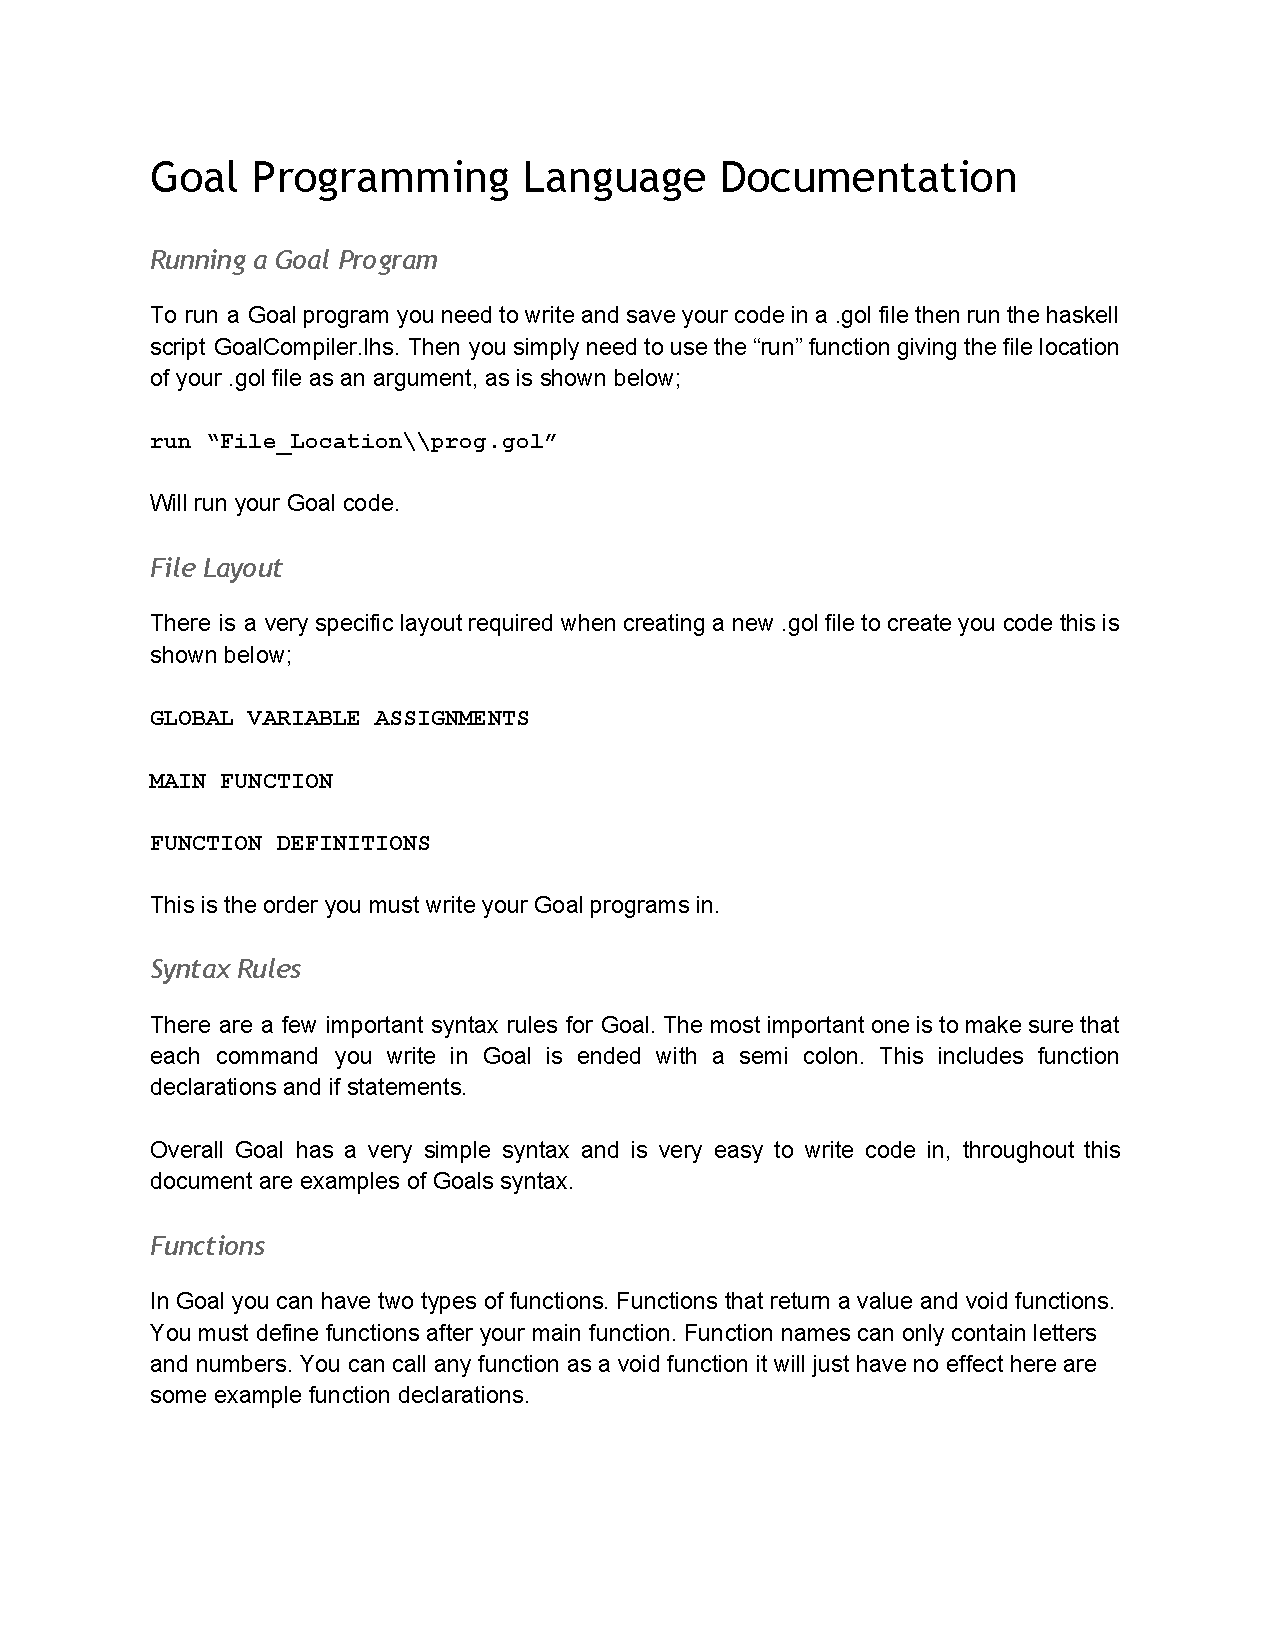
\includepdf[pages={1-7}]{GoalDocumentation.pdf}

\chapter{Referenced Code}
\section{Parsing.lhs}
\lstinputlisting[basicstyle=\tiny,]{Parsing.lhs}

\chapter{My Code}

\section{GoalCompiler.lhs}
\lstinputlisting[basicstyle=\tiny,]{GoalCompiler.lhs}

\section{GoalParser.lhs}
\lstinputlisting[basicstyle=\tiny,]{GoalParser.lhs}

\section{GoalMachine.lhs}
\lstinputlisting[basicstyle=\tiny, breaklines=true,]{GoalMachine.lhs}

\bibliographystyle{plainnat}
\bibliography{Bibliography}

\end{document}

